% Literal captions copied from their source inputs by build_complete_continuation_article.py.
% Native PowerPoint sources and reviewed PNG pixels remain unchanged.
\begin{figure*}[p]
\centering
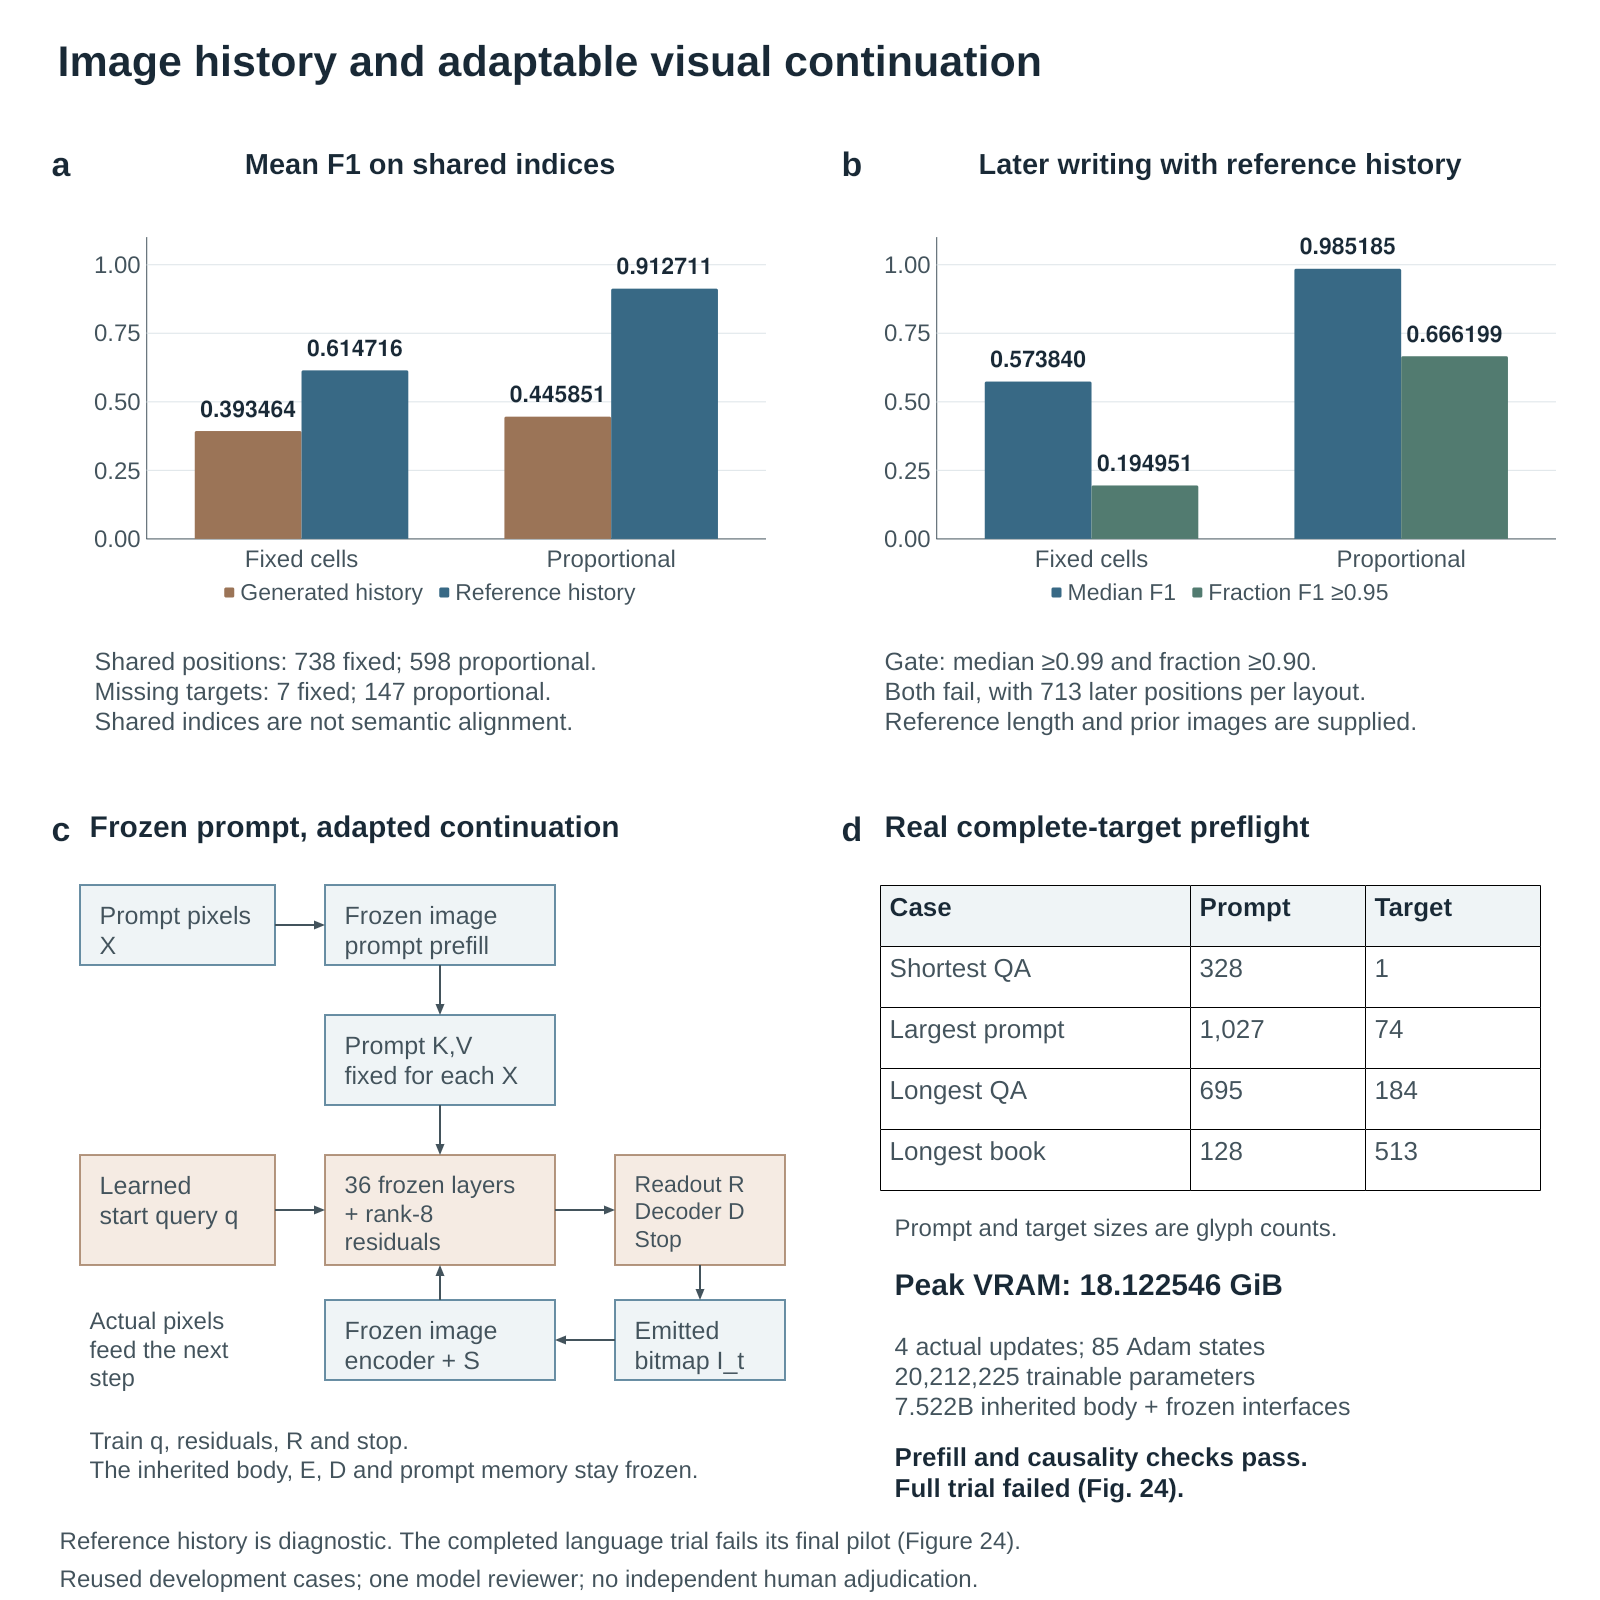
\includegraphics[width=.92\textwidth]{figures/Figure_23_continuation_history_completed.png}
\caption{\textbf{Correct prior images improve canonical writing without qualifying autonomous language.}
\textbf{a}, Mean foreground F1 at target indices present under both generated
and supplied reference-image history: 738 fixed-layout and 598 proportional
positions. Missing and extra autonomous positions remain in the complete
records. Numeric index agreement does not align alternative semantic answers.
Reference history supplies answer information and length, with stopping bypassed.
\textbf{b}, Median later F1 and the fraction of later positions reaching 0.95,
using all 713 later reference positions per layout. Both layouts fail the joint
median/count gate. These canonical image metrics are not language accuracies.
\textbf{c}, Implemented continuation computation. Frozen prompt prefill creates
immutable prompt keys and values. The query and all 36 native answer layers
continue from visible glyph images; new residuals, readout and stopping train,
while the inherited body, image encoder/decoder and affine transform remain
frozen. The stopping head is separate from decoded pixels. Only actually emitted
images supply subsequent inputs; every answer layer is recomputed during fitting.
\textbf{d}, Four complete preflight cases retain all 772 target positions and
four terminal boundaries. Four real optimizer updates peak at 18.122546\,GiB
allocated GPU memory. Independent audits check targets, optimizer states and
numerical boundaries; prompt/frozen-body checks come from the registered GPU
execution. Initial residual-down tensors were not archived in that preflight.
The 7.522B inherited body and frozen interfaces remain deployed costs beyond
the 20,212,225 trainable parameters. F1 chart cells and labels round to six
decimals; complete precision remains in bound records. The supplied-history
diagnosis and preflight are separate from the completed full fit, whose final
language pilot fails (Fig.~24). The later joint writer
has no measured language result here. Reused development data and one model
reviewer with prior familiarity lack independent human adjudication or untouched
confirmation.}
\label{fig:continuation-history}
\end{figure*}
\begin{figure*}[p]
\centering
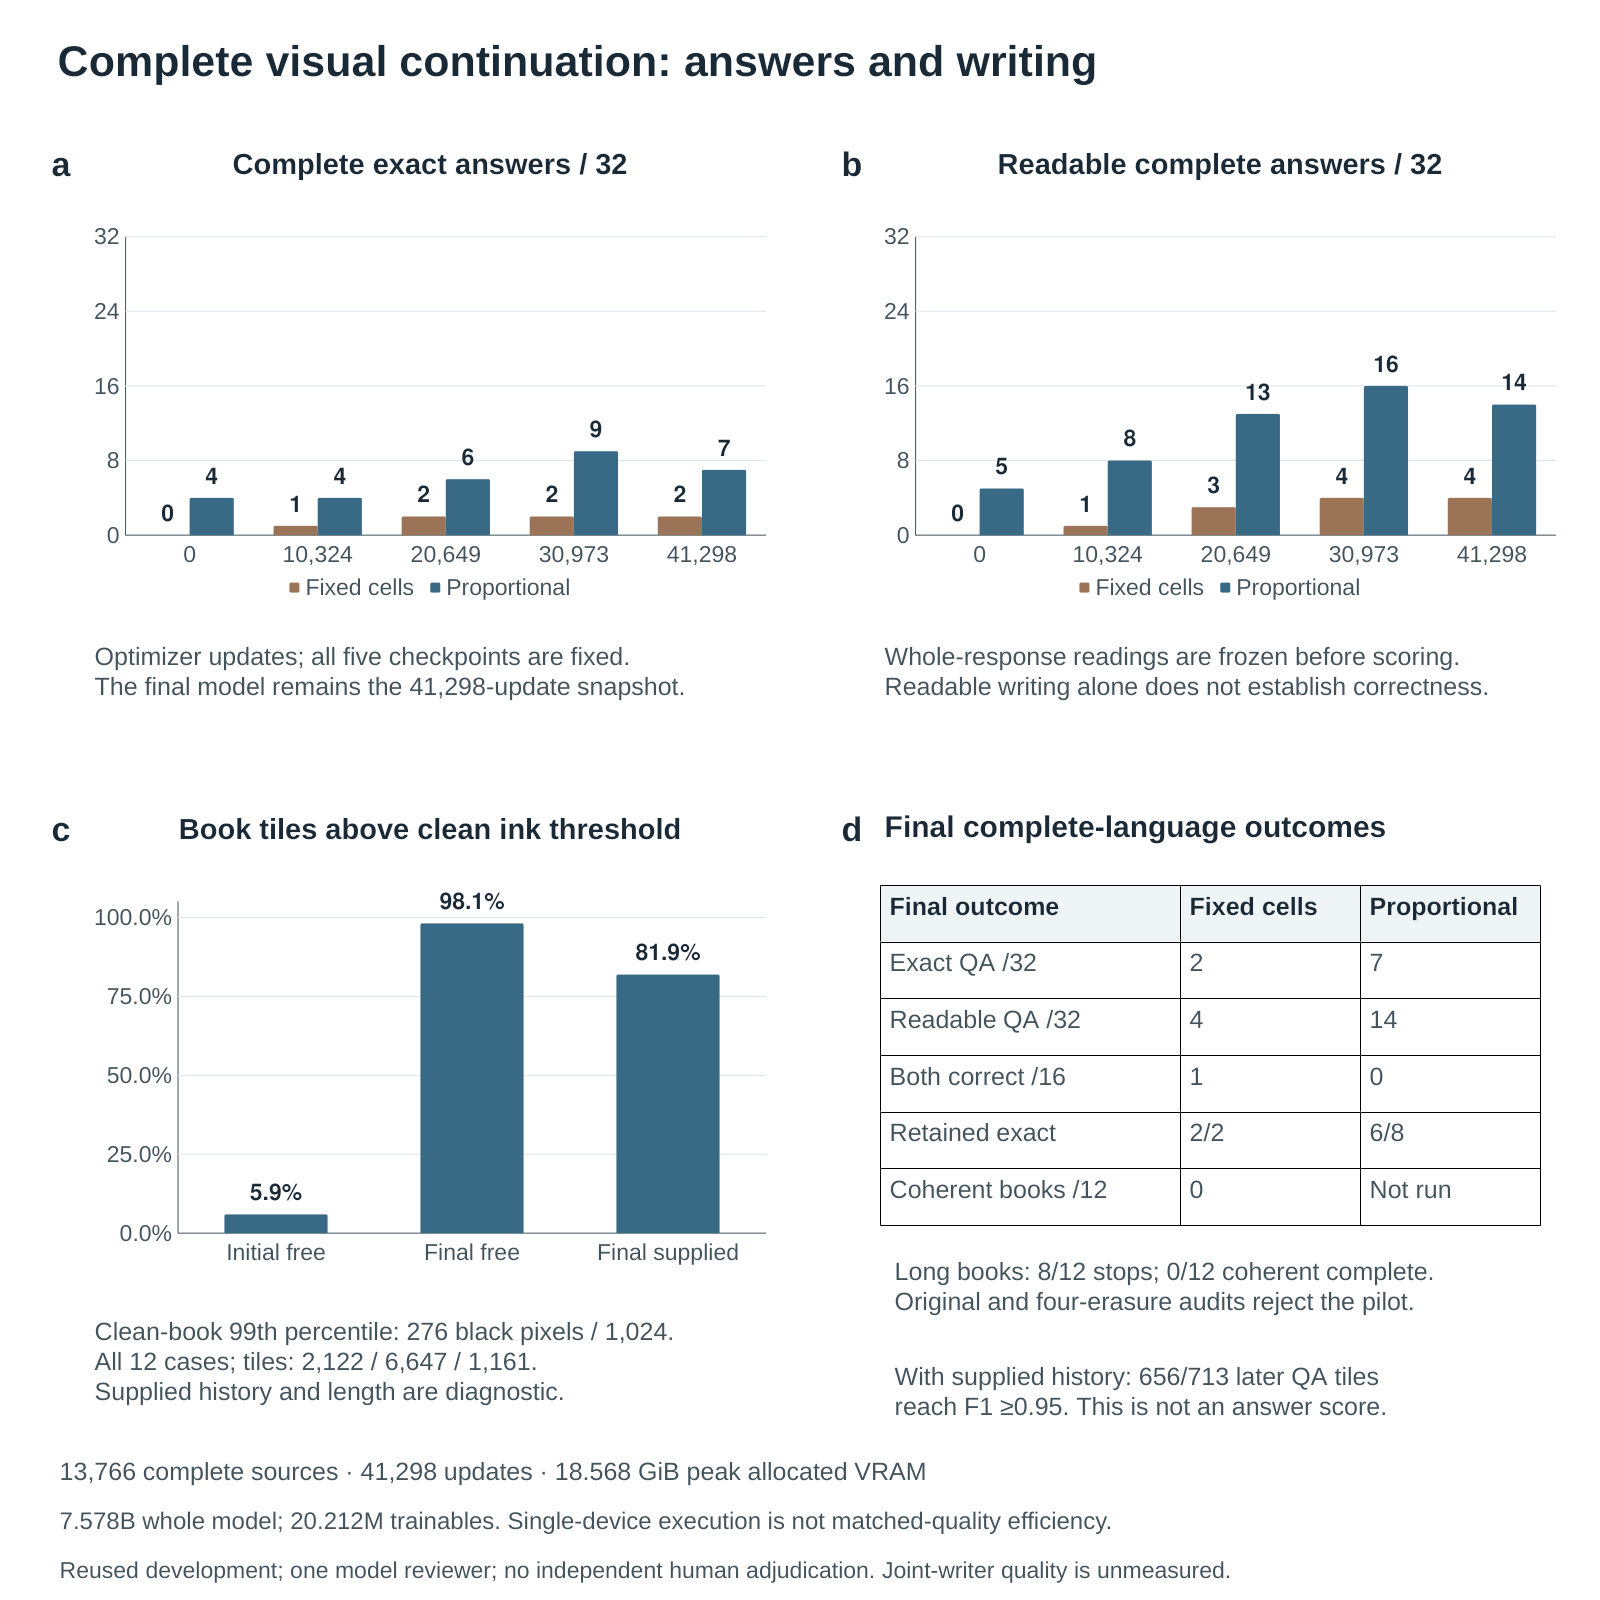
\includegraphics[width=.92\textwidth]{figures/Figure_24_complete_continuation.png}
\caption{\textbf{Complete visual-continuation adaptation improves some short answers
but fails sustained writing.}
\textbf{a,b,} Frozen whole-response exact and readable counts at all five fixed
checkpoints, with 32 questions and sixteen paired passage groups per layout.
The three-quarter peak does not replace the prescribed final model.
\textbf{c,} Fractions of book tiles above the clean training-book 99th-percentile
ink count, 276 of 1,024 pixels. Initial and final autonomous pools contain 2,122
and 6,647 tiles; the final supplied-history pool contains 1,161 target positions.
Each pool retains all twelve prefixes, but lengths differ. Supplied preceding
answer images and length, with stopping bypassed, make the third bar a physical
diagnosis. Chart fractions round to six decimals for workbook storage and percent
labels to one decimal; exact counts and full precision remain in the
source data. Excess ink alone does not establish its cause or a stable attractor.
\textbf{d,} Final complete-answer, paired and retained-success counts. Book prompts
use only the fixed layout; no normal book arm receives a coherent complete
continuation. The 656/713 later QA positions reaching F1 0.95 use supplied history
and do not replace autonomous answer scores. Both the original pilot and the
four-QA-erasure audit reject the final model. The full deployment retains
7.578 billion parameters; one-GPU execution does not establish a matched-quality
efficiency advantage. All results use reused development data and one model
reviewer, with no independent human adjudication. The subsequent joint writer
has no language result in this figure.}
\label{fig:complete-continuation}
\end{figure*}
\begin{figure*}[p]
\centering
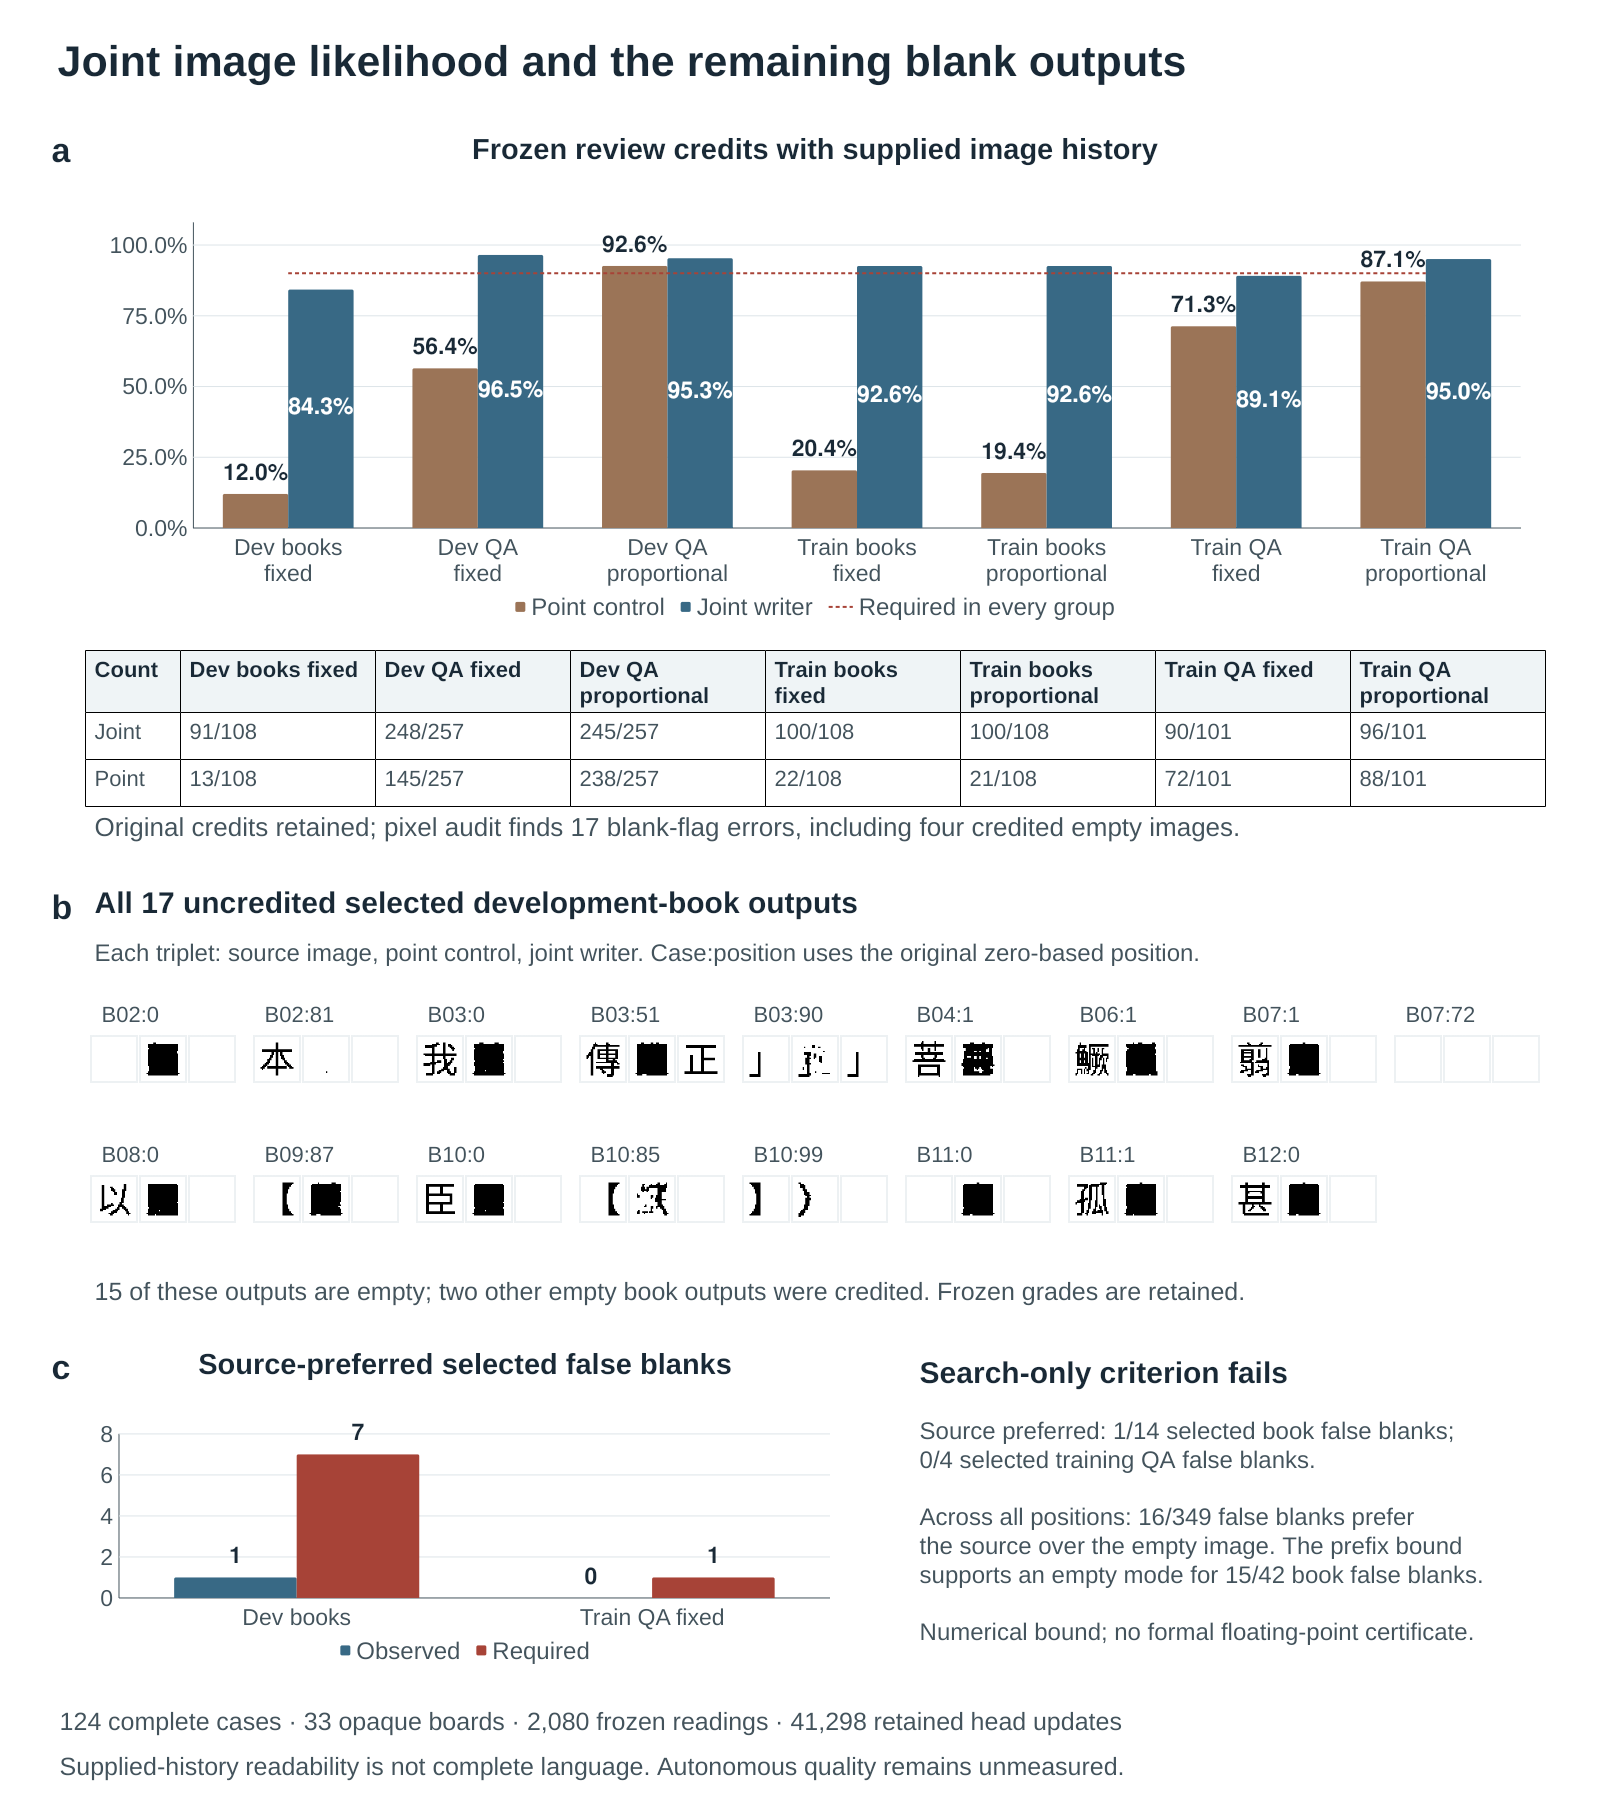
\includegraphics[width=.92\textwidth]{figures/Figure_25_joint_writer_physical.png}
\caption{\textbf{Joint image likelihood changes conditional writing but fails physical qualification.}
\textbf{a,} Original frozen readability credits for the joint writer and unchanged point-writer control in all seven supplied-history groups. The dashed line is the prespecified 90\% prerequisite for every candidate group. Exact counts accompany the chart; chart fractions are rounded to six decimal places. Development books and training QA with fixed cells fail. These are retained review counts, not corrected physical accuracy: a subsequent pixel audit finds 17 blank-flag disagreements among 2,080 readings, including four credited empty images. \textbf{b,} Every uncredited selected development-book output, ordered by case and original zero-based position. Each triplet shows the source, point control and joint output. Original binary $32\times32$ images are expanded threefold by nearest neighbour, without repair. Fifteen of these seventeen joint outputs are empty and two are nonempty; two other empty book outputs were credited. Among all 108 selected book positions, four source images are blank, three overlapping the seventeen empty outputs, giving fourteen false blanks. \textbf{c,} Complete-image likelihood prefers the source over the empty image for one of fourteen selected book false blanks and none of four selected training-QA false blanks, below the unchanged requirements of seven and one. Across all 12,597 positions, sixteen of 349 false blanks prefer their source; the prefix bound supports an empty mode in fifteen of 42 development-book false blanks. The finite-precision bound is not a formal certificate. Review used one model reviewer with prior cohort familiarity and no independent human adjudication. Frozen readings, original scores and the failed verdict are preserved. Autonomous language quality remains unmeasured.}
\label{fig:joint-writer-physical}
\end{figure*}
